\chapter{DENKLEM, RESİM, ALGORİTMA ÖRNEKLERİ}
Istanbul is a beautiful city of stunning architecture, history and culture. You'll find ancient and modern colleges, fascinating museums and galleries, and plenty of parks, gardens and green spaces in which to relax. Although the city is spread over a large area, you will have easy reach to anywhere you would like to go thanks to a variety of modern and developed transportation systems as well as interchangeable rail systems to long-way metrobus lines.

\begin{figure}[!htbp]
\centering
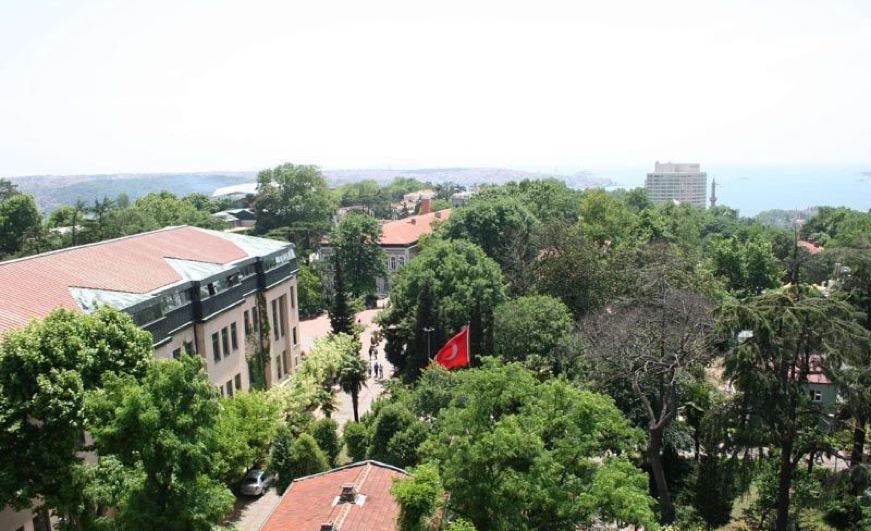
\includegraphics[width=\textwidth]{thesisChapters/images/Picture1.png}
\caption{Landscape design of Yıldız Technical University}
\label{fig:landscape}
\end{figure}

In Figure \ref{fig:landscape}, landscape design of Yıldız Technical University is illustrated.

\section{History}
The stages our university has passed through in its distinguished past are outlined below. Kondüktör Mekteb-i Âlisi/ The Conductors (Technicians) School of Higher Education (1911-1922). The Kondüktör Mekteb-i Âlisi/Conductors (Technicians) School of Higher Education was founded in 1911 in order to meet the “science officer” (known previously as conductors, and today as technicians) requirement of the Municipality Public Works Section. The school was modeled on the syllabus of the “Ecole de Conducteur” and was affiliated with the Ministry of Public Works. Enrolment began on 22 August 1911. Harita ~\ref{fig:itu} de İTÜ haritasıdır.

\begin{map}[!htbp]
\centering
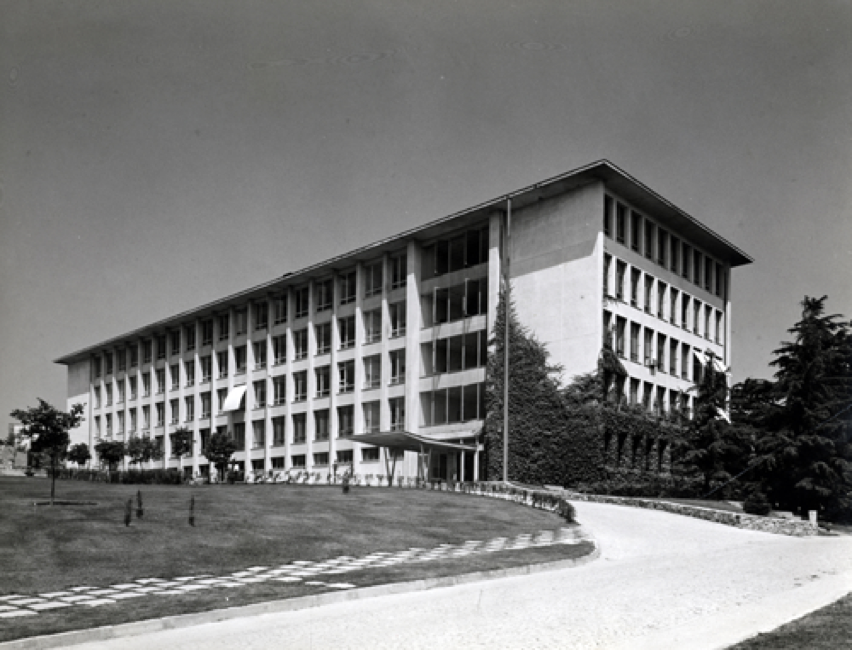
\includegraphics[width=\textwidth]{thesisChapters/images/Picture2}
%\includegraphics[scale=0.6]
\caption{The Istanbul Technical School}
\label{fig:itu}
\end{map}

\textbf{Nafia Fen Mektebi/ The School of Public Works (1922-1937):}  The school’s name was changed to Nafia Fen Mektebi/ School of Public Works in 1922 and the duration of education was increased to 2.5 years in 1926 and 3 years in 1931.

\section{Historical Advancements in the University}

The school was established as an autonomous higher education and research institution with Law no. 1184 of State Engineering and Architectural Academies published on 3 June 1969. 

Law no. 1472 ruled for the closing of special vocational schools in 1971, and engineering schools were affiliated with the Istanbul State Engineering and Architectural Academy.

\subsection{The Yıldız University Period}
The Istanbul State Engineering and Architectural Academy and affiliated schools of engineering and the related faculties and departments of the Kocaeli State Engineering and Architecture Academy and the Kocaeli Vocational School were merged to form Yıldız University with decree law no.41 dated 20 June 1982 and Law no. 2809 dated 30 March 1982 which accepted the decree law with changes.

The new university incorporated the departments of Science-Literature and Engineering, the Vocational School in Kocaeli, a Science Institute, a Social Sciences Institute and the Foreign Languages, Atatürk Principles and the History of Revolution, Turkish Language, Physical Education and Fine Arts departments affiliated with the Rectorate.

\subsection{The Yıldız Technical University Period}
Law no. 3837 dated 3 July 1992 renamed our university Yıldız Technical University. The Engineering Faculty was divided into four faculties and restructured as the Electrical-Electronics, Construction, Mechanical and Chemical-Metallurgy Faculties and also included the Faculty of Economics and Administrative Sciences within its organization. The Kocaeli Faculty of Engineering and the Kocaeli Vocational School were released from our university to be restructured as Kocaeli University. Today our university has 9 Faculties \footnote{2 of these faculties are located at Yildiz Campus, and the other ones are located at Davutpaşa Campus}, 2 Institutes, the Vocational School of Higher Education, the Vocational School for National Palaces and Historical Buildings, the Vocational School for Foreign Languages and more than 20,000 students . 

\begin{figure}[htbp]
\centering
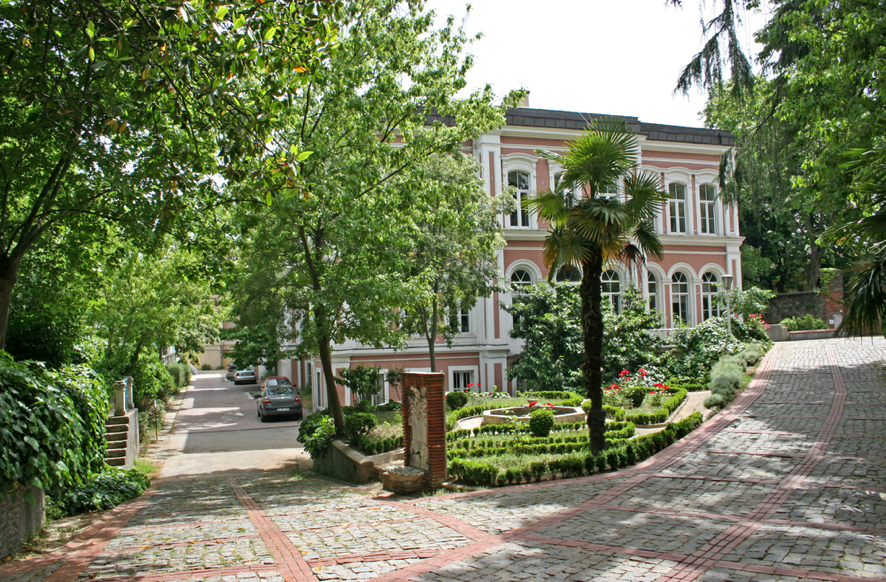
\includegraphics[width=\textwidth]{thesisChapters/images/Picture3}
\caption{Side view of Graduate School of Natural and Applied Sciences, Yıldız Technical University, Çukursaray, İstanbul [10]}
\end{figure}

\subsubsection{Mission}
Our mission is to create a university which pioneers education, scientific research, technological development and artistic work aimed at the progress of society and the increase of the quality of life within an understanding of national and international solidarity; and educates creative, enterprising, questioning and ethical students equipped with universal values, who constantly renew themselves, aim for lifelong learning and are capable of analysis and synthesis.

\begin{equation}
\Delta  l = h \Delta \theta
\end{equation}
\begin{equation}
\frac{\Delta l}{\Delta t} = h \frac{\Delta \theta}{\Delta t}
\end{equation}
\begin{equation}
\lim_{\Delta t \rightarrow 0}\frac{\Delta l}{\Delta t} = \lim_{\Delta t \rightarrow 0} h \frac{\Delta \theta}{\Delta t}
\end{equation}
\begin{equation}
\lim_{\Delta t \rightarrow 0}\frac{\Delta l}{\Delta t} = \frac{dI}{dt}
\end{equation}

Here's more complex formula example.

\subsection{Skip-gram}
Skip-gram metodunda bir kelime girilir ve daha sonra belirli pencere etrafındaki kelimeler tahmin ettirilir. Tek bir girdi değerinden etrafındaki kelimeri çıktı olarak alabiliyoruz. Skip-gram modeli, verilen corpus'a göre her kelimenin kelime vektörlerini eğitir. Cümle içinde bir kelime \textit{(W(t))} verildiğinde,mevcut kelimenin \textit{W(t)} olasılığıyla. skip-gram, yakındaki $w_{i}(t-k\leqslant i\leqslant t + k)$ kelimelerinin \textit{P(W(t+i)|W(t))} olasılıklarını tahmin edebilir.Her sözcük vektörü yakındaki kelimelerin konumlarını yansıtır. Skip-gram modelinin amacı aşağıdaki değeri en üst düzeye çıkarmaktır:

\begin{equation}
    \centering
    E=\frac{1}{n}\sum\limits_{t=1}^{n}{\left(\sum\limits_{-k\le i\le k,i\ne 0}{{{log}_{2}}P(W(t+i)|W(t))} \right)}
\end{equation}


\section{Algoritma gösterimi}

Algoritma örnekleri tablo olarak alınır. Tablo \ref{model}'de görüldüğü üzere programlama diline göre format gösterimi, satır numarası gösterimi mümkündür.

\begin{lstlisting}[language=python, caption=Construction of the Model , label=model]
from keras.datasets import imdb
from keras import models
from keras.callbacks import ModelCheckpoint
from keras import layers
from keras import optimizers
from keras import losses
from keras.callbacks import EarlyStopping, ModelCheckpoint
from keras.models import load_model
import csv
import matplotlib.pyplot as plt
import pandas as pd
import numpy as np
import sys
import argparse

\end{lstlisting}

\section{Tablo örnek}

Tablo \ref{phardesc}'de tablo başlığı boyalı halde gösterilmiştir.

\begin{table}[!ht]
\caption{Cavity Point Features and Pharmacophore Matching Rules}
\centering
\begin{tabular}{l l l l}
\rowcolor{gray!25}
\toprule
\textbf{Property}    &\textbf{Name}  &\textbf{Residue}     &\textbf{Closest Protein Atom} \\ 
\midrule
Hydrophobic(HYD)    &CA   &Gly    &Hydrophobic        \\ 
Aromatic(AR)     &CZ  &Phe    &Aromatic                \\ 
Acceptor(HBA)   &O    &Ala    &Donor                   \\ 
Donor(HBD)      &N   &Ala     &Acceptor      \\ 
Acceptor/Donor(HBAD)  &OG   & Ser      &Acceptor/Donor \\ 
Positive Ionizable(D+)  &NZ   & Lys    &Negative Ionizable    \\ 
Negative Ionizable(A-)  &OD1   & Asp   &Positive Ionizable     \\ 
Null(DU)  &DU   &Cub      &None     \\ 
\bottomrule
\end{tabular}
\label{phardesc}
\end{table}
